\begin{question}
\noindent A game designer is creating a symmetrical map layout for a Valorant-style level. Triangle $M$ marks the position of one team's spawn zone, as shown on the grid below.

\begin{center}
\scalebox{0.85}{%
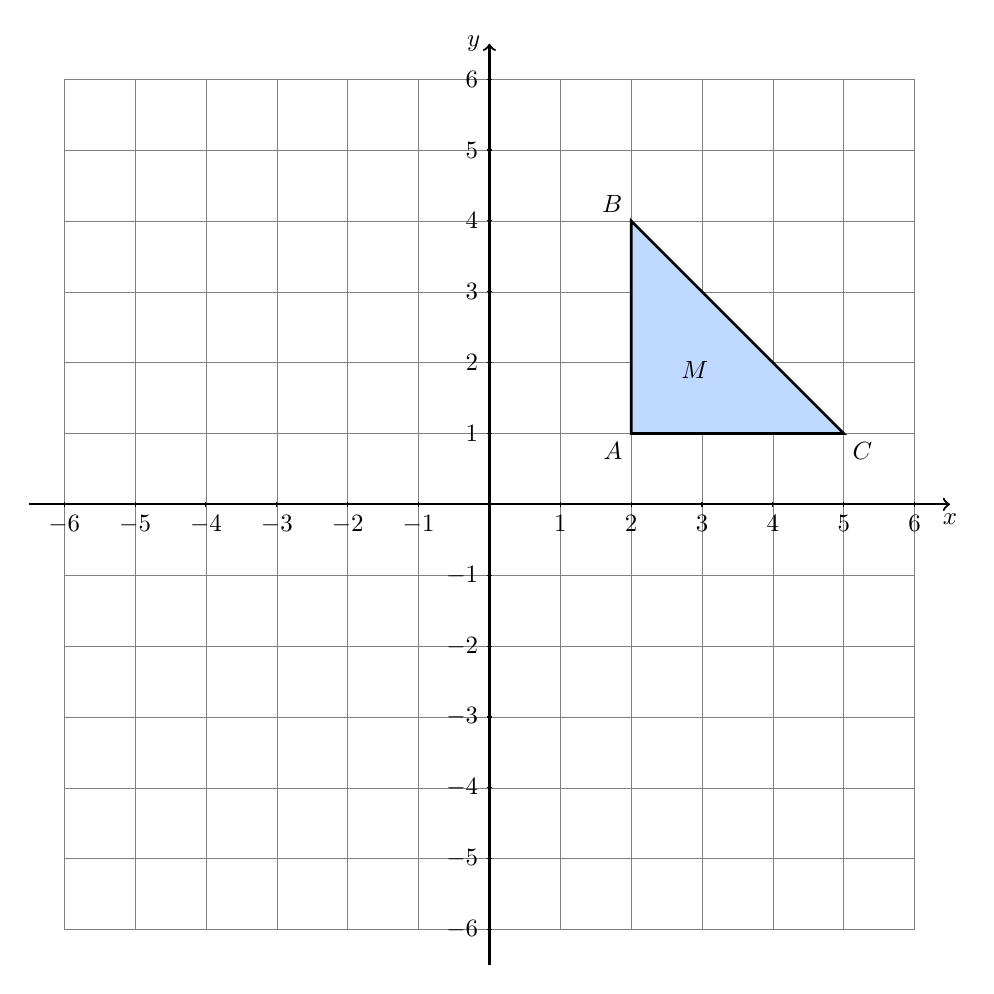
\begin{tikzpicture}[scale=0.9, transform shape]
    \definecolor{borderColour}{HTML}{000000}
    \definecolor{fillColourM}{HTML}{BFD8FF}

    \def\axisLimit{6}

    % Draw grid
    \draw[step=1cm,gray,very thin] (-\axisLimit,-\axisLimit) grid (\axisLimit,\axisLimit);

    % Draw axes
    \draw[thick,->] (-\axisLimit-0.5,0) -- (\axisLimit+0.5,0) node[anchor=north] {$x$};
    \draw[thick,->] (0,-\axisLimit-0.5) -- (0,\axisLimit+0.5) node[anchor=east] {$y$};

    % Label x-axis and y-axis
    \foreach \x in {-\axisLimit,...,-1,1,2,...,\axisLimit}
        \draw (\x cm,1pt) -- (\x cm,-1pt) node[anchor=north] {$\x$};
    \foreach \y in {-\axisLimit,...,-1,1,2,...,\axisLimit}
        \draw (1pt,\y cm) -- (-1pt,\y cm) node[anchor=east] {$\y$};

    % Triangle M: A(2,1), B(2,4), C(5,1)
    \coordinate (A) at (2,1);
    \coordinate (B) at (2,4);
    \coordinate (C) at (5,1);
    \filldraw[fill=fillColourM, draw=borderColour, line width=1pt] (A) -- (B) -- (C) -- cycle;

    \node[below left] at (A) {$A$};
    \node[above left] at (B) {$B$};
    \node[below right] at (C) {$C$};
    \node at (2.9,1.9) {$M$};

\end{tikzpicture}%
}
\end{center}

\noindent Reflect triangle $M$ in the $x$-axis.\\
Label the image $N$.

\vspace{4cm}

\begin{flushright}
    \answerplain{2}
\end{flushright}
\end{question}